% Capítulo 7: matriz 3 x 4 com linhas e colunas, e como ela fica na memória.
\documentclass[border=4pt]{standalone}
\usepackage[utf8]{inputenc}
\usepackage[T1]{fontenc}
% Estilo comum das figuras de vetores (capítulo 8).
\usepackage{tikz}
\usetikzlibrary{arrows.meta, positioning, calc, decorations.pathreplacing}
\definecolor{navy}{RGB}{23,45,80}
\definecolor{laranja}{RGB}{250,110,29}
\definecolor{cinzalogo}{RGB}{107,114,126}
\definecolor{azul}{RGB}{205,222,247}
\tikzset{
  casa/.style={draw=navy, line width=0.9pt, minimum width=8mm, minimum height=7mm,
               inner sep=0pt, font=\sffamily\small},
  pronta/.style={casa, fill=azul},
  parte/.style={casa, fill=laranja!12},
  marcada/.style={casa, fill=laranja!45, draw=laranja},
  fora/.style={casa, draw=cinzalogo!60, dashed, fill=white, text=cinzalogo!60},
  indice/.style={font=\sffamily\scriptsize, text=cinzalogo},
  explica/.style={font=\sffamily\small, text=navy, anchor=east},
  legenda/.style={font=\sffamily\scriptsize, text=cinzalogo},
  rotulo/.style={font=\sffamily\small\bfseries, text=navy},
  seta/.style={-{Stealth[length=2.2mm]}, navy, line width=0.9pt},
  chave/.style={decorate, decoration={brace, amplitude=4pt, mirror}, navy, line width=0.8pt},
}
% \vetor{nome}{x}{y}{valor/estilo, valor/estilo, ...}: casas lado a lado, chamadas nome0, nome1...
\newcommand{\vetor}[4]{%
  \foreach \valor/\estilo [count=\i from 0] in {#4} {
    \node[\estilo] (#1\i) at ($(#2, #3) + (\i*0.8, 0)$) {\valor};
  }
}

\tikzset{
  casa/.append style={minimum width=10mm, minimum height=7mm},
  mini/.style={draw=navy, line width=0.7pt, minimum width=6mm, minimum height=6mm, inner sep=0pt, font=\sffamily\scriptsize},
}
\begin{document}
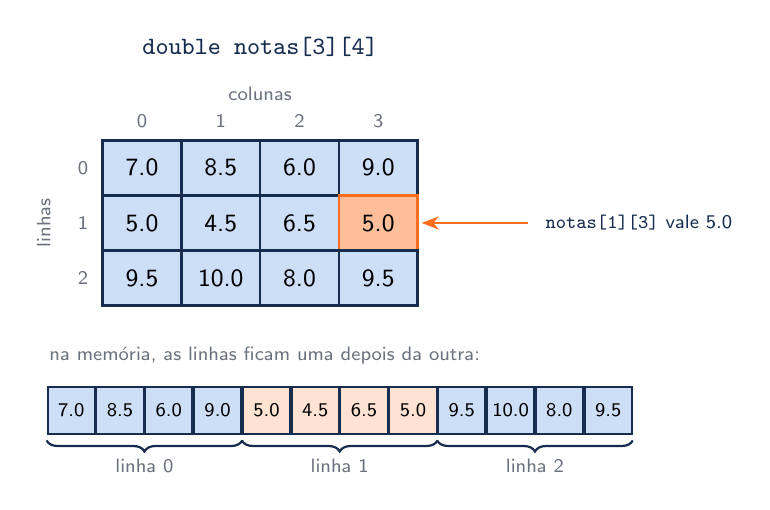
\begin{tikzpicture}[x=10mm, y=7mm]
  % a matriz
  \foreach \linha [count=\i from 0] in {{7.0,8.5,6.0,9.0},{5.0,4.5,6.5,5.0},{9.5,10.0,8.0,9.5}} {
    \foreach \v [count=\j from 0] in \linha {
      \ifnum\i=1 \ifnum\j=3
        \node[marcada] at (\j, -\i) {\v};
      \else
        \node[pronta] at (\j, -\i) {\v};
      \fi \else
        \node[pronta] at (\j, -\i) {\v};
      \fi
    }
    \node[indice] at (-0.75, -\i) {\i};
  }
  \foreach \j in {0,...,3} { \node[indice] at (\j, 0.85) {\j}; }
  \node[indice] at (1.5, 1.35) {colunas};
  \node[indice, rotate=90] at (-1.25, -1) {linhas};
  \node[rotulo] at (1.5, 2.2) {\texttt{double notas[3][4]}};
  \draw[seta, laranja] (4.9, -1) -- (3.55, -1);
  \node[legenda, text=navy, anchor=west] at (5.0, -1) {\texttt{notas[1][3]} vale 5.0};

  % na memória
  \node[legenda, anchor=west] at (-1.3, -3.4) {na memória, as linhas ficam uma depois da outra:};
  \foreach \v [count=\k from 0] in {7.0,8.5,6.0,9.0,5.0,4.5,6.5,5.0,9.5,10.0,8.0,9.5} {
    \pgfmathtruncatemacro{\lin}{int(\k/4)}
    \ifnum\lin=1
      \node[mini, fill=laranja!20] (m\k) at (-0.9 + \k*0.62, -4.4) {\v};
    \else
      \node[mini, fill=azul] (m\k) at (-0.9 + \k*0.62, -4.4) {\v};
    \fi
  }
  \draw[chave] ($(m0.south west)+(0, -0.1)$) -- node[below=3pt, legenda] {linha 0} ($(m3.south east)+(0, -0.1)$);
  \draw[chave] ($(m4.south west)+(0, -0.1)$) -- node[below=3pt, legenda] {linha 1} ($(m7.south east)+(0, -0.1)$);
  \draw[chave] ($(m8.south west)+(0, -0.1)$) -- node[below=3pt, legenda] {linha 2} ($(m11.south east)+(0, -0.1)$);
\end{tikzpicture}
\end{document}
